%~Mouliné par MaN_auto v.0.23.0 2020-05-18 14:08:49
\documentclass[AHL,Unicode,longabstracts]{cedram}

%%\usepackage{amssymb}
%%\usepackage{amsfonts}
%\usepackage{amsthm}
%\usepackage{amsmath}
%%\usepackage{mathtools}
%%\usepackage{graphicx}
\usepackage{mathtools}

\makeatletter
\def\@altabstractlanguage{}
\makeatother

\newcommand*{\dd}{\mathrm{d}}
\newcommand*{\dx}{\dd x}
\newcommand*{\dy}{\dd y}
\newcommand*{\dz}{\dd z}
\newcommand*{\du}{\dd u}
\newcommand*{\dv}{\dd v}
\newcommand{\sdots}{{\mk.\mK.\mK.\mK}}
\newcommand{\scdots}{{\mk{\cdot}\mK{\cdot}\mK{\cdot}\mk}}

\newcommand*{\myangle}{\mathord{\langle}} %~ \langle est une pseudo parenthèse mais l'auteur l'utilise comme un symbole ordinaire. Il faut donc changer son type pour corriger les problèmes d'espace avec les +, -, etc.

\newcommand*{\I}{\textsl{I}}
\newcommand*{\II}{\textsl{II}} % pour mieux gérer les espaces entre les I

%\usepackage{amscd}


\DeclareMathOperator{\airy}{Airy} 
\DeclareMathOperator{\hit}{hit} 
\DeclareMathOperator{\shk}{shk} 
\DeclareMathOperator{\tw}{TW} 
\DeclareMathOperator{\err}{Err} 
\DeclareMathOperator{\hypo}{hypo} 
\DeclareMathOperator{\tr}{tr} 
\DeclareMathOperator{\hs}{HS} 
\DeclareMathOperator{\op}{op} 
\DeclareMathOperator{\Ai}{Ai}
\DeclareMathOperator{\argl}{arg} 
\DeclareMathOperator{\const}{const} 


\newcommand{\E}[1]{\mathbf{E}\left[#1\right]}
\newcommand{\pr}[1]{\mathbf{Pr}\left[#1\right]}
\newcommand{\ind}[1]{\mathbf{1}_{\{ #1 \}}}
\newcommand{\eps}{\varepsilon}
\newcommand{\Z}{\mathbb{Z}}
\newcommand{\R}{\mathbb{R}}
%%\newcommand{\Ai}{\mathrm{Ai}}
\newcommand{\A}{\mathcal{A}}
\newcommand{\h}{\mathfrak{h}}

%%%%%%%%%%%%%%%%%%%%%%%%%%%%%%%%%%%%%%%%%%%%%%%%%%%%%%%%%%%%%%%%%%%%
\providecommand{\noopsort}[1]{}
\graphicspath{{./figures/}}

\newcommand*{\mk}{\mkern -1mu}
\newcommand*{\Mk}{\mkern -2mu}
\newcommand*{\mK}{\mkern 1mu}
\newcommand*{\MK}{\mkern 2mu}

\hypersetup{urlcolor=purple, linkcolor=blue, citecolor=red}

\newcommand*{\romanenumi}{\renewcommand*{\theenumi}{\roman{enumi}}}
\newcommand*{\Romanenumi}{\renewcommand*{\theenumi}{\Roman{enumi}}}
\newcommand*{\alphenumi}{\renewcommand*{\theenumi}{\alph{enumi}}}
\newcommand*{\Alphenumi}{\renewcommand*{\theenumi}{\Alph{enumi}}}
%%%%%%%%%%%%%%%%%%%%%%%%%%%%%%%%%%%%%%%%%%%%%%%%%%%%%%%%%%%%%%%%%%%%

\title{TASEP fluctuations with soft-shock initial data}
\alttitle{Fluctuations TASEP avec données initiales à choc modéré}

\keywords{Burgers equation, exclusion process, KPZ universality, shock fluctuations, Tracy--Widom law}
\subjclass{60K35, 46N30, 82C22, 82C23}


\author{\firstname{Jeremy} \lastname{Quastel}}
\address{Department of Mathematics,\\
University of Toronto,\\
Toronto, ON (Canada)}
\email{quastel@math.toronto.edu}

\author{\firstname{Mustazee} \lastname{Rahman}}
\address{Department of Mathematics,\\
Massachusetts Institute of Technology,\\
Cambridge, MA (USA)}
\address{\tralicstex{}{\emph{and}\\}
Department of Mathematical Sciences,\\
Durham University,\\
Durham (UK)}
\email{mustazee@gmail.com}


\editor{A. Debussche}


\begin{abstract}
We consider the totally asymmetric simple exclusion process with \emph{soft-shock} initial particle density, which is a step function increasing in the direction of flow and the step size chosen small to admit KPZ scaling. The initial configuration is deterministic and the dynamics create a shock.

We prove that the fluctuations of a particle at the macroscopic position of the shock converge to the maximum of two independent GOE Tracy--Widom random variables, which establishes a conjecture of Ferrari and Nejjar. Furthermore, we show the joint fluctuations of particles near the shock are determined by the maximum of two lines described in terms of these two random variables. The microscopic position of the shock is then seen to be their difference.

Our proofs rely on determinantal formulae and a novel factorization of the associated kernels.
\end{abstract}

\begin{altabstract}
On considère le processus d'exclusion simple totalement asymétrique avec une densité initiale de particules à \emph{choc modéré}, ayant la forme d'une fonction en escalier qui augmente dans la direction du flux et dont le saut est choisi suffisamment petit pour satisfaire l'échelle KPZ. On suppose que la configuration initiale est déterministe et que la dynamique crée un choc.

On montre que les fluctuations d'une particule située à l'endroit macroscopique du choc convergent vers le maximum de deux variables aléatoires indépendantes de type GOE Tracy--Widom. Ceci prouve une conjecture de Ferrari et Nejjar. On montre également que les fluctuations conjointes des particules près du choc sont décrites par le maximum de deux lignes définies en termes de ces deux variables aléatoires. La position microscopique du choc apparaît alors comme leur différence.

Nos preuves sont basées sur des formules déterminantes et une nouvelle factorisation des noyaux associés.
\end{altabstract}

\datereceived{2018-08-09}
\daterevised{2019-02-27}
\dateaccepted{2019-10-14}

%%%%%%%%%%%%%%%%%%%%%%%%%%%%%%%%%%%%%%%%%%%%%%%%%%%%%%%%%%%%%%%%%%%%

\begin{document}


\maketitle

\section{Introduction}

The continuous time totally asymmetric simple exclusion process (TASEP) is an interacting particle system on an one-dimensional lattice. At time zero, there is a given initial configuration of particles such that every site of $\Z$ occupies at most one particle. The dynamics are as follows. A particle jumps randomly to its neighbouring site to the right provided that it is empty. The jumps of a particle are independent of the others' and performed with exponential waiting times having mean 1.

The observables in TASEP are the positions of particles. Initially, particles are numbered by integers in increasing order from right to left with particle 1 being the first one to the left of the origin. Denote by $X_t(n)$ the position of particle number $n$ at time $t$. Thus, given the initial configuration $X_0({\,\cdot\,})$, particles are numbered such that
\[
\dots < X_0(3) < X_0(2) < X_0(1) < 0 \leq X_0(0) < X_0(-1) < X_0(-2) < \cdots.
\]
By convention, if there is a rightmost particle then $X_0(n) = + \infty$ for every $n$ after that particle, and similarly, $X_0(n) = - \infty$ for every $n$ preceding a leftmost particle. As an example, if the initial configuration occupies all sites at the negative integers then $X_0(1) = -1, X_0(2) = -2, X_0(3) = -3$ and so on, while $X_0(0) = X_0(-1)= \dots = + \infty$.

A detailed construction and basic features of TASEP are given in~\cite{Lig}. The model can also be seen as a randomly growing one-dimensional interface whose gradient is the particle density. In this respect it belongs to the Kardar--Parisi--Zhang (KPZ) universality class. The surveys~\cite{BG, Q} discuss the relationship of TASEP to KPZ.

Despite its simplicity TASEP displays many of the interesting behaviour of non-equilibrium statistical mechanics. Consider a deterministic initial configuration such that the macroscopic particle density is $\rho_{-}$ to the left of the origin and $\rho_{+}$ to the right:
\begin{equation}\label{eqn:ID}
\rho_{\pm} = \lim_{t \to \, \infty}\; \frac{\# \, \{\text{particles in the interval} \; [0, \pm t]\;\text{at time}\;0\}}{t}\,.
\end{equation}
For instance, particles may be arranged periodically in large enough blocks to attain such a profile. On the macroscopic scale the evolution of the particle density is a solution to Burgers' equation~\cite{R, S3}. Namely, for every $T > 0$ there is a density $u(T,x)$ such that
\[
\int _a^b u(T,x) \, \dx = \lim_{t \to \, \infty}\; \frac{\# \, \{\text{particles in the interval} \; [at, bt]\;\text{at time}\; Tt\} }{t} \;\; \text{almost surely},
\]
and $u$ is the unique entropy solution of Burgers' equation:
\begin{equation}\label{eqn:Burgers}
\partial_T u + \partial_x (u (1-u)) = 0, \quad u(0,x) = \rho_{-} \ind{x < 0} + \rho_{+} \ind{x \geq 0}.
\end{equation}

When $\rho_{-} < \rho_{+}$, there is a traffic jam in the system because particles to the left of the origin, moving at macroscopic speed $1-\rho_{-}$, run into particles to the right of the origin moving at a slower speed of $1-\rho_{+}$. In this case the relevant solution of~\eqref{eqn:Burgers} is given by the travelling front
\[
u(T,x) = u(0, x-\nu T), \;\; \text{where}\;\; \nu = 1- \rho_{-} - \rho_{+}\,.
\]

The number $\nu$ is the speed of the traffic jam. This is the shock in Burgers' equation. It is of interest to study the microscopic features of the shock, ergo, the fluctuations of TASEP with an initial particle configuration as above.

\begin{figure}[t]
\begin{center}
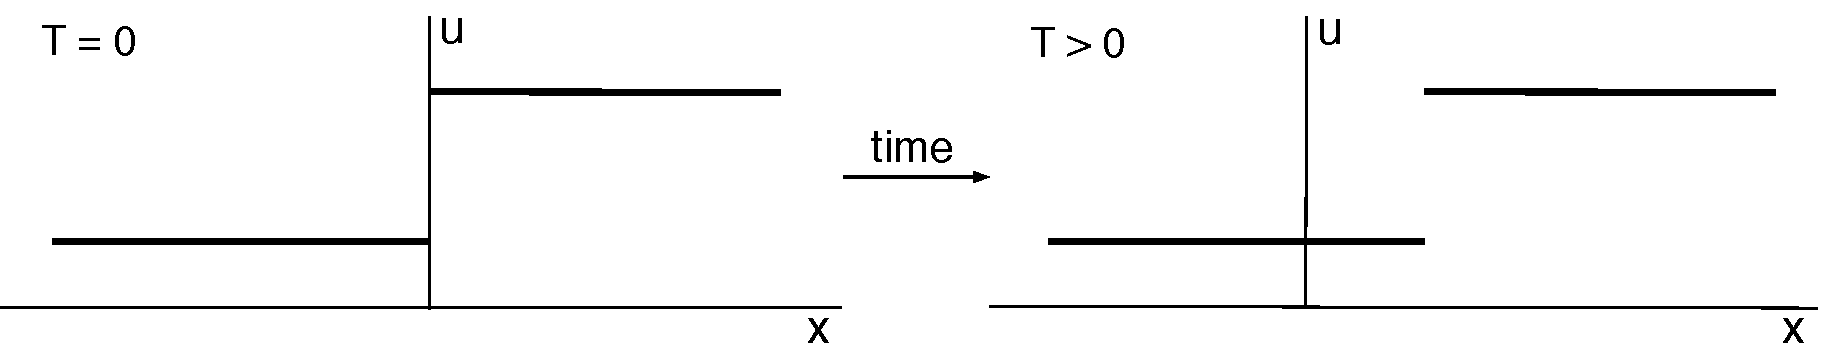
\includegraphics[scale=0.45]{shockwave.pdf}
\caption{The travelling shock-front $u(T,x)$ that solves~\eqref{eqn:Burgers}.}
\end{center}
\end{figure}

A proxy for the location of the shock is the particle at macroscopic position $\nu t$. For large times, the number\footnote{Rounding particle numbers to nearest integers is omitted throughout the paper.} of said particle is
\[
n^{\shk}_t = (\rho_{-} \rho_{+})t \,.
\]
Its position fluctuates randomly to the order $t^{1/3}$ and one would like to calculate, for every $a \in \R$,
\[
\lim_{t \to \, \infty}\, \pr{ X_t \big(n^{\shk}_t \big) \geq \nu t - a t^{1/3}}\,.
\]

\subsection{The soft shock} This paper considers a softening of the shock where the parameters $\rho_{\pm}$ are scaled~as
\begin{equation}\label{eqn:softrho}
\rho_{\pm} = \frac{1 \pm \beta (t / 2)^{-1/3}}{2},\;\; \beta \in \R \;\;\text{and}\;\; t \geq 2|\beta|^{3}.
\end{equation}
In the soft shock scenario, TASEP is run until time $t$ with the choice of $\rho_{\pm}$ as in~\eqref{eqn:softrho} and $t$ being the parameter within $\rho_{\pm}$. One then considers the law of $X(n^{\shk}_t)$ in the double limit as $t \to \infty$ followed by $\beta \to \infty$, in order to transition into the shock.

\begin{theo} \label{thm:1}
Consider TASEP with a deterministic initial configuration of particles having macroscopic density as in~\eqref{eqn:ID} and $\rho_{\pm}$ scaled as in~\eqref{eqn:softrho}. Then,
\[
\lim_{\beta \to \infty}\; \lim_{t \to \infty}\, \pr{X_t \big(n^{\shk}_t \big) \geq - a t^{1/3}} = F_1(2a)^2,
\]
where $F_1$ is the distribution function of the GOE Tracy--Widom law.
\end{theo}

The soft shock is introduced in~\cite{FN2} and Theorem~\ref{thm:1} proves a conjecture there. The scaling~\eqref{eqn:softrho} is considered ``critical'' for TASEP since the resulting particle fluctuations belong to the KPZ universality class with regards to their scaling exponents and limit laws. Interestingly, as remarked in Section~\ref{sec:shockremarks}, the large time limit of the soft shock recovers many of the universal Airy processes ($\airy_1$, $\airy_2$, etc.) through various limit transitions of the parameter $\beta$. Also, the rate of convergence that we find in Theorem~\ref{thm:1} is of order $\beta^{-1}$, although this is not optimized.

The advantage of the soft shock is that it allows to transition into the hard shock by means of exact calculation of statistical laws. More precisely, one can describe the limiting law of $X_t(n^{\shk}_t)$ as $t \to \infty$ in terms of Fredholm determinants. Indeed, Theorem~\ref{thm:2} provides the large $t$ limiting joint distribution of particles that are in the window of the soft shock, and Theorem~\ref{thm:3} establishes the large $\beta$ limit of that. Together, they imply Theorem~\ref{thm:1}. These methods should also apply to prove GOE Tracy--Widom cubed, quadrupled, etc., limiting laws at the merger of shocks when the initial particle density has two jumps, three jumps, and so on. We do not pursue it here.

\subsection{Large time limit of the TASEP with soft shock} In the case of soft shock the particle numbered $n^{\shk}_t$ has non-trivial correlations with other particles that are within a distance of order $t^{2/3}$ of its position. Their positions fluctuate on a scale of order $t^{1/3}$. As such, consider particles having numbers
\[
n(t, x) = n^{\shk}_t - x(t/2)^{2/3} = \frac{t}{4} - \frac{\beta^2}{2}(t/2)^{1/3} - x(t/2)^{2/3},
\]
for $x \in \R$, which at time $t$ have macroscopic positions
\[
m(t,x) = \frac{x (t/2)^{2/3}}{\rho_{-}} = \frac{2x}{1-\beta(t/2)^{-1/3}}\, (t/2)^{2/3}.
\]
The first limit transition derives the large $t$ limit of the process
\begin{equation}\label{eqn:firstlim}
x \, \mapsto \, \frac{X_t(n(t,x)) - m(t,x)}{-(t/2)^{1/3}}\,.
\end{equation}

\begin{theo}\label{thm:2}
Given real numbers $x_1 < x_2 < \dots < x_m$ and $a_1, \dots, a_m$, as $ t \to \infty$,
\[
\pr{ X_t(n(t,x_i)) \geq m(t,x_i) - a_i(t/2)^{1/3},\; 1 \leq i \leq m}
\]
converges to
\[
\pr{ \h(1,x_i \,; \, 2\beta|y|) \leq \beta^2 - 2\beta x_i + a_i, \; 1 \leq i \leq m},
\]
where $\h(1,x; 2\beta|y|)$ is a random function of the variable $x$. The multi-point distribution functions of $\h(1,x; 2\beta |y|)$ are given in terms of Fredholm determinants:
\begin{align*}
& \pr{\h(1,x_i \,;\, 2\beta|y|) \leq a_i,\; 1\leq i \leq m}\\
& =\det\!\left (I \Mk-\Mk e^{-x_m \partial^2}K_{\beta}e^{x_m \partial^2}
\big (I \Mk-\Mk e^{(x_1-x_m)\partial^2}\bar{\chi}_{a_1} e^{(x_2-x_1)\partial^2} \bar{\chi}_{a_2}
\cdots e^{(x_m-x_{m-1})\partial^2}\bar{\chi}_{a_m} \big)\right)_{L^2(\R)},
\end{align*}
where $\bar{\chi}_{a}(u) = \ind{u \leq a}$ is projection onto $L^2(-\infty, a)$ and $K_{\beta}$ is an explicit operator.
\end{theo}
$K_{\beta}$ is defined separately in Section~\ref{sec:softkernel} since its introduction requires crucial terminology and concepts.

Complicated though the determinant in Theorem~\ref{thm:2} may appear, observe the one-point distribution functions of $\h(1,x; 2\beta |y|)$ are given by the Fredholm determinant of operators $e^{-x\partial^2} K_{\beta} e^{x \partial^2}$ over the spaces $L^2(a,\infty)$. These will turn out simpler and play a crucial role in the proofs.

The reason we call the limit process $\h(1,x; 2\beta |y|)$ is that it is the height function at time $1$ of the KPZ fixed point with initial data $h_0(y) = 2\beta|y|$, as introduced in~\cite{MQR}. The KPZ fixed point refers to what is expected to be the asymptotic scaling invariant Markov process for the KPZ universality class. Although the KPZ fixed point motivates our paper to an extent, the kernels in this case were actually known previously in~\cite{FN2}, and so the results used from~\cite{MQR} are somewhat auxiliary.

\subsection{Transition into the shock}
The main result of the paper is the large $\beta$ limit law of the process $\h(1,x; 2\beta|y|)$.
\begin{theo} \label{thm:3}
As $\beta \to \infty$, the process
\[
x \mapsto \, \h \big (1, (2\beta)^{-1} x \, ; \, 2 \beta |y| \big) - \beta^2
\]
converges in the sense of finite dimensional laws to the process
\begin{equation}\label{limitprocess}
x \mapsto \, \max \{ \, 2^{-2/3} X_{\tw_1} - x,\, 2^{-2/3} X'_{\tw_1} + x \, \},
\end{equation}
where $X_{\tw_1}$ and $X'_{\tw_1}$ are two independent GOE Tracy--Widom random variables.
\end{theo}

Stated in terms of the TASEP soft shock, Theorem~\ref{thm:3} asserts that in the double limit of $t \to \infty$ followed by $\beta \to \infty$ the process
\[
x \, \mapsto \, \frac{X_t \big (n(t,(2\beta)^{-1}x) \big) - \beta^{-1}x(t/2)^{2/3}}{-(t/2)^{1/3}}
\]
converges in law to the process~\eqref{limitprocess}. Process~\eqref{limitprocess} may be thought of as the asymptotic ``shock process'' of TASEP with initial density~\eqref{eqn:ID}.

\begin{figure}[htpb]
\begin{center}

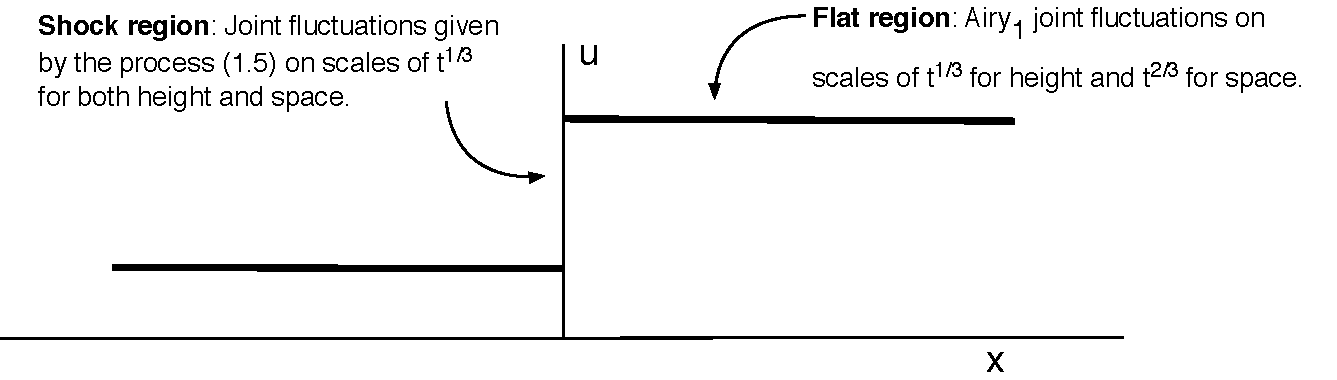
\includegraphics[scale=0.6]{flucsummary.pdf}
\caption{Fluctuations of TASEP that arise from initial density~\eqref{eqn:ID} when $\rho_{\pm}$ are given by~\eqref{eqn:softrho}.}\label{fig:2}
\end{center}
\end{figure}

\begin{rema*}[on interpretation of Theorem~\ref{thm:3}]
The process~\eqref{limitprocess} may be expressed as $|x- X| + Y$ with $X = (X_{\tw_1} - X'_{\tw_1})/2^{5/3}$ and $Y = (X_{\tw_1} + X'_{\tw_1})/2^{5/3}$. As this process represents the asymptotic position of particles around the shock, the ``microscopic density'' near the shock may be interpreted as its derivative, which is simply an increasing step function with jump at $X = (X_{\tw_1} - X'_{\tw_1})/2^{5/3}$. The \emph{microscopic position} of the shock is then at $X$, and one finds the TASEP shock to be rigid in that the microscopic density remains a step with the randomness only affecting its microscopic location.
\end{rema*}

\subsection{Remarks on the soft shock process} \label{sec:shockremarks}
``Soft shock'' is bit of a misnomer since the shock manifests for large values of $\beta$ whereas the process in Theorem~\ref{thm:2} has interesting features for negative values of $\beta$ as well. We have a family of processes interpolating from the $\airy_2$ process at $\beta = -\infty$ to the process~\eqref{limitprocess} at $\beta = + \infty$. This is easily seen from the framework of the aforementioned KPZ fixed point, as the mapping from initial data $h_0$ to $\h(1,x; h_0)$ is continuous, so long as $h_0$ is upper semicontinuous with values in $[-\infty, \infty)$ and bounded from above by a linear function.

When $\beta = 0$, $\h(1,x; 0)$ is the $\airy_1$ process corresponding to flat initial data $h_0 \equiv 0$. As $\beta \to - \infty$, the function $2\beta|y|$ converges to $- \infty \, \ind{y \neq 0}$, which is called the narrow wedge or droplet ($-\infty \times 0 = 0$). Then $\h(1,x; 2\beta |y|)$ converges to $\h(1,x; \, \text{narrow\;wedge})$, which has the law of the $\airy_2$ process minus a parabola. Its distribution at $x = 0$ is the GUE Tracy--Widom law.

The soft shock also interpolates between two $\airy_1$ processes at $x = -\infty$ and $x = \infty$. Indeed, affine and translation symmetries of the KPZ fixed point~\cite[Theorem~4.5]{MQR} imply that for constants $c$ and $u$,
\[
\h \big(1,x+u; h_0(y) \big) -c(x+u)-\frac{c^2}{4} \;\overset{\text{law}}{=}\;
\h \bigg(1,x; \, h_0 \Big (y+u+\frac{c}{2} \Big) - c \Big (y+u+\frac{c}{2} \Big) \bigg).
\]
Thus, $\h(1,x \pm L; \, 2\beta|y|) - \beta^2 \mp 2\beta(x \pm L)$ has the same law as $\h (1,x; \,4 \beta (x \pm (\beta+L))_{\mp})$. The latter processes converge to $\h(1,x;\, \text{flat})$ as $L \to \infty$.

One can also find the $\airy_{2 \to 1}$ process, which is the law of $\h (1,x; \, - \infty \cdot \ind{y < 0})$. The initial data is called half-flat. Indeed, $\h (1,x+\beta; \, 2\beta|y|) - \beta^2 + 2\beta(x+\beta)$ has the law of $\h (1,x; \, 4\beta (y)_{-})$, and $4\beta (y)_{-}$ converges to the half-flat function as $\beta \to - \infty$.

\subsection{An overview of the proof} \label{sec:overview}
It is well known that the correlation functions of TASEP, which provide the probability of particles being at specific sites, are determinantal; see for instance~\cite{BFPS, BG} and references there. Our proofs rely on such formulae.

Let us summarize how the GOE TW-squared law arises in Theorem~\ref{thm:1}. The operator $K_{\beta}$ whose Fredholm determinant provides the law of $h(1,0;2\beta |y|)$ can be \emph{factorized} as
\[
I-K_{\beta} = (I - M_{\beta} K_0M^{-1}_{\beta}) \cdot (I - M^{-1}_{\beta} K_0 M_{\beta}) + \err_{\beta}.
\]
$\err_{\beta}$ is an error term that is vanishingly small in the appropriate trace norm as $\beta \to \infty$. This effectively allows us to consider the Fredholm determinant of the product. That approximately becomes a product of determinants, and then the conjugations by $M_{\beta}$ can be removed. This results in the GOE TW-squared law in the large $\beta$ limit.

Observe that if one conjugates away $M_{\beta}$ from one of the factors in the above representation then the other factor is conjugated by $M^2_{\beta}$, and the resulting operator, $M^{\pm2}_{\beta}K_0 M^{\mp2}_{\beta}$, does not in fact converge as $\beta \to \infty$. This was a challenge faced in previous works.

\subsection{Review of literature} \label{sec:lit}
The study of the TASEP shock has a history and the reader may find nice discussions in~\cite{F2, FFV} and their references. We provide an overview of prior works most directly related to ours.

In~\cite{BFS} the authors find determinantal formulae for TASEP with particles having varying speeds, which allows them to study shock fluctuations with Bernoulli-random initial data. The fluctuations there are Gaussian to the order of $t^{1/2}$. The papers~\cite{BC, CFP, FFV} have related results for Bernoulli initial data. Deterministic shock-like initial data is studied in~\cite{FN1, FN3} by connecting TASEP to last passage percolation. The authors prove that shock fluctuations for various setups are governed by the maximum of various Tracy--Widom random variables, although they are unable to treat the step initial density~\eqref{eqn:ID}.

The soft shock is introduced in~\cite{FN2} in a setup where particles move at two different speeds instead of being spread out with the two densities $\rho_{\pm}$. The authors prove the analogue of our Theorem~\ref{thm:2}, and present determinantal kernels for the multi-point distributions in terms of contour integrals. One may verify that their kernel matches ours. They also conjecture our Theorem~\ref{thm:1}. A beautiful illustration of the convergence of $X_t(n^{\shk}_t)$ to the GOE TW-squared law is shown in~\cite[Figure~1]{FN2}. The paper~\cite{N} also considers a scenario like the soft shock but with narrow-wedge-like initial data.

Finally, it is well known that for the general asymmetric simple exclusion process, when started with Bernoulli--random initial data modelling the step density~\eqref{eqn:ID}, a second class particle from the origin follows the macroscopic shock for large times $t$ and has asymptotically Gaussian fluctuations to the order $t^{1/2}$; see e.g.~\cite{Lig}. However, when~\eqref{eqn:ID} is modelled by deterministic initial data, \cite{FGN} proves that the asymptotic position of the second class particle in TASEP is the difference of two independent GOE Tracy--Widom random variables on the scale of $t^{1/3}$. One may think of the second class particle as a random walk in the potential well given by the TASEP height process, and so it should sit at the minimum of process~\eqref{limitprocess}, which is indeed $(X_{\tw_1}- X'_{\tw_1})/2^{5/3}$. Further discussions about shocks in ASEP have appeared in~\cite{BB, N2} after this paper.

\subsection*{Acknowledgements}
JQ was supported by the Natural Sciences and Engineering Research Council of Canada. MR is thankful to Alexei Borodin for helpful discussions and guidance during early stages of this work. The authors also thank Patrik Ferrari for a valuable discussion as well as Ivan Corwin, Promit Ghosal and Daniel Remenik for their comments.

\section{The soft shock operator} \label{sec:softkernel}

The operator $K_{\beta}$ associated to the soft shock is defined in terms of operators
\begin{equation}\label{eqn:S}
S_x = \exp \left\{x \partial^2 + \frac{1}{3}\partial^3\right\}, \;\;\text{for}\; x \in \R,
\end{equation}
acting on functions $f \in L^2(a,\infty)$ for any fixed $a >-\infty$. (Recall the notation $e^L = \sum_{k \geq 0} \frac{L^k}{k!}$. For instance, translation by $\lambda$ is $e^{\lambda \partial}$ since $f(x + \lambda) = \sum_{k \geq 0} \frac{\partial^k f(x)}{k!} \lambda^k$; its integral kernel is $e^{\lambda \partial}(u,v) = \delta_{u+\lambda,v}$.)

The operator $\exp \{x \partial^2\}$, which corresponds to the heat kernel, is ill-defined for $x < 0$ but $S_x$ is well-defined due to the presence of the third derivative operator. In terms of integral kernels,
\begin{equation}\label{eqn:Skernel}
S_x(u,v) = e^{\frac{2}{3}x^3 + x(v-u)} \Ai(v-u + x^2),
\end{equation}
where $\Ai(z)$ is the Airy function defined as
\begin{equation}\label{eqn:Aifunc}
\Ai(z) = \frac{1}{2 \pi \mathbf{i}} \, \oint_{\myangle} \dd w \, e^{\frac{w^3}{3} - z w},
\end{equation}
and $\myangle$ is a contour consisting of two rays going from $e^{-\mathbf{i} \pi/3} \infty$ to $e^{\mathbf{i} \pi/3} \infty$ through 0. (The Airy function also satisfies the Airy equation $\Ai'' (x) = x \Ai(x)$ with $\Ai(x) \to 0$ as $x \to + \infty$.) The operator $S_0$ will often be denoted $S$. We will use the fact that
\[
S^{*} S = S S^{*} = I.
\]

We now introduce the important \emph{hitting operator}. Let $B(y)$, for $y \geq 0$, denote a Brownian motion with diffusion coefficient 2. Let $h : [0,\infty) \to [-\infty, \infty)$ be upper semicontinuous with at most linear growth in the sense that $h(y) \leq C (1+ |y|)$ for some constant $C$. Let
\[
\tau = \inf \, \{ y \geq 0: B(y) \leq h(y)\}.
\]
Define the operator $S^{\hypo(h)}_x$ in terms of its integral kernel as
\begin{equation}\label{eqn:hypokernel}
S^{\hypo(h)}_x(u,v) = \E{S_{x-\tau}(B(\tau),v)\ind{\tau < \infty} \,\middle|\, B(0) = u}.
\end{equation}
If $u \leq h(0)$ then $S^{\hypo(h)}_x = S_x$. If $h$ is continuous and $u > h(0)$ then
\[
S^{\hypo(h)}_x(u,v) = \E{S_{x-\tau}(h(\tau),v)\ind{\tau < \infty} \,\middle|\, B(0) = u}.
\]
Consider also the projection operators onto $L^2(a,\infty)$ and $L^2(-\infty, a)$, respectively:
\begin{equation}\label{eqn:proj}
\chi_a(u,v) = \ind{u = v, \,u > a} \quad \text{and} \quad \bar{\chi}_a = 1 - \chi_a.
\end{equation}

The hitting operator is defined as follows. Consider an upper semicontinuous $h : \R \to [-\infty, \infty)$ that has at most linear growth. The hitting operator associated to $h$ requires choosing a \emph{split point} $x \in \R$. Then consider the functions
\[
h^{\pm}_x(y) = h(x \pm y) \quad \text{for}\;\; y \geq 0.
\]
The hitting operator is
\begin{equation}\label{eqn:hitkernel}
K^{\hypo(h)} = I - \left (S_x - S^{\hypo(h^{-}_x)}_x \right)^{*} \chi_{h(x)}
\left (S_{-x} - S^{\hypo(h^{+}_x)}_{-x}\right).
\end{equation}
It is a crucial property of the hitting operator that it does not depend on the choice of split point $x$ (see~\cite{QR1} for a proof).

The operator $K_{\beta}$ is the hitting operator associated to $h_{\beta}(y) = 2\beta |y|$. It is natural (and crucial for the large $\beta$ asymptotics) to take the split point at $x = 0$, which utilizes the fact that $h_{\beta}$ has different slopes on the two sides of the split point. Denoting $h^{+}_{\beta}(y) = 2 \beta y$ for $y \geq 0$,
\begin{equation}\label{eqn:Khypo}
I - K_{\beta} = \left (S - S^{\hypo(h^{+}_{\beta})}\right)^{*} \chi_0
\left (S - S^{\hypo(h^{+}_{\beta})}\right)\,.
\end{equation}
Since $S^{*} S = I$, $K^{\hypo(h_{\beta})}$ can be expressed as
\[
S^{*} \bar{\chi}_0S \,+\, S^{*} \chi_0 S^{\hypo(h^{+}_{\beta})} \,+\, (S^{\hypo(h^{+}_{\beta})})^{*} \chi_0 S \,-\,
(S^{\hypo(h^{+}_{\beta})})^{*} \chi_0 S^{\hypo(h^{+}_{\beta})}.
\]
Each of these terms have a presence of the operator $\exp \{ \pm \, \partial^3/3 \}$ on both sides. This ensures that the operator $\exp\{ x \partial^2\}$ can be applied legally around $K^{\hypo(h_{\beta})}$ for every $x \in \R$, and so the operator inside the determinant from the statement of Theorem~\ref{thm:2} is well-defined.

For general initial data $h_0$, the multi-point distribution functions of $\h(1,x; h_0)$ are given as follows. Given $x_1 < \dots < x_m$ and $a_1, \dots, a_m$,
%\begin{multline}\label{eqn:KPZjoint}
%\pr{\h (1,x_i; h_0) \leq a_i\,;\, 1 \leq i \leq m} \\
%=\det\!\left(\!I\Mk\!-\!e^{-x_m \partial^2}\! K^{\hypo(h_0)}e^{x_m \partial^2}
%\!\big(\!I\Mk\!-\!e^{(x_1-x_m)\partial^2}\mk\bar{\chi}_{a_1} e^{(x_2-x_1)\partial^2}\mk \bar{\chi}_{a_2}
%\scdots\MK e^{(x_m-x_{m-1})\partial^2} \bar{\chi}_{a_m}\!\big)\!\right)\!_{L^2(\R)}.
%\end{multline}
\begin{multline}\label{eqn:KPZjoint}
\pr{\h (1,x_i; h_0) \leq a_i\,;\, 1 \leq i \leq m} \\
=\det\Big(I-e^{-x_m \partial^2} K^{\hypo(h_0)}e^{x_m \partial^2}
\big(I-e^{(x_1-x_m)\partial^2}\bar{\chi}_{a_1} e^{(x_2-x_1)\partial^2} \bar{\chi}_{a_2}\\
\cdots e^{(x_m-x_{m-1})\partial^2} \bar{\chi}_{a_m}\big)\Big)_{L^2(\R)}.
\end{multline}

The determinantal expression for the multi-point distribution function is the ``path integral'' version from~\cite{MQR}. There is an alternative ``extended kernel'' version. The hitting operator is also introduced in~\cite{QR1} in a modified form and precursors appear in~\cite{BCR, CQR, PS, QR3}.

\section{First limit transition: proof of Theorem~\ref{thm:2}} \label{sec:KPZlimit}

Let us introduce a parameter $\eps > 0$ and write
\[
t = 2 \eps^{-3/2}.
\]
Then $m(t,x) = 2x \eps^{-1} + 2\beta x \eps^{-1/2} + O(\beta^2)$. The events of interest are
\[
X_{2 \eps^{-3/2}}\left(\frac{1}{2}\eps^{-3/2} -x\eps^{-1} - \frac{\beta^2}{2} \eps^{-1/2}\right) \geq
2x \eps^{-1} + (2\beta x -a)\eps^{-1/2} + O(\beta^2).
\]
In order to prove Theorem~\ref{thm:2} one must derive the limiting joint probabilities of such events as $\eps \to 0$. Upon replacing $x$ with $x - (\beta^2/2)\eps^{1/2}$ the event becomes
\begin{equation}\label{eqn:softevent}
X_{2 \eps^{-3/2}}\Big(\frac{1}{2}\eps^{-3/2} -x\eps^{-1}\Big)
\geq 2x \eps^{-1} - \big(\beta^2 - 2\beta x + a \big)\eps^{-1/2} + O(\beta^2).
\end{equation}

We may express the event~\eqref{eqn:softevent} in terms of the height function of TASEP. For TASEP with initial data $X_0$, let
\[
X_t^{-1}(u) = \min\, \{n \in \Z: X_t(n) \leq u\}.
\]
The height function $h_t: \Z \to \Z$ at time $t$ is
\[
h_t(z) = -2 \big (X_t^{-1}(z-1) - X_0^{-1}(-1) \big) - z.
\]
The KPZ-rescaled height function is
\begin{equation}\label{eqn:KPZh}
h^{\eps}(T,x) = \eps^{1/2} \left [h_{2T\eps^{-3/2}}(2x\eps^{-1}) + T \eps^{-3/2} \right].
\end{equation}
In terms of the KPZ-rescaled height function one has
\[
h^{\eps}(T,x) \leq a \;\Longleftrightarrow\;
X_{2T\eps^{-3/2}}\bigg(\frac{T}{2}\eps^{-3/2} - x\eps^{-1}\bigg) \geq 2x\eps^{-1} - a \eps^{-1/2} + X_0(1).
\]
In the $\eps \to 0$ limit the probability of the event in~\eqref{eqn:softevent} remains unaffected if the term $O(\beta^2)$ is ignored. Thus, one must show that the limiting multi-point probabilities
\[
\lim_{\eps \to 0}\, \pr{ h^{\eps}(1,x_i) \leq \beta^2 - 2\beta x_i +a_i, \; 1\leq i \leq k}
\]
are given by the formula from Theorem~\ref{thm:2}. (The function $h^{\eps}(0,y)$ converges uniformly to $h_0(y)= 2\beta |y|$.)

Here there are several approaches. In~\cite{FN2}, a determinantal formula is derived for these multi-point probabilities for the soft-shock data in a related setup, where particles to the left of the origin have a different speed than those to the right. Using their formula, it is not difficult to guess a determinantal formula for our setup and then check it using the bi-orthogonalization procedure from~\cite{BFPS, Sas}. On the other hand, \cite[Theorem~2.6]{MQR} provides a formula for any initial data with a rightmost particle. One can cutoff the soft-shock initial data far to the right and take a limit as the cutoff is removed to get a determinantal formula for the multi-point probabilities which coincides with the guess. Then by direct asymptotic analysis of the associated determinantal kernels one arrives at Theorem~\ref{thm:2}. This is done with generality in~\cite[Theorem~3.13]{MQR} (``Convergence of TASEP''). Since the limiting kernel is the same as~\cite{FN2}, we omit the details.

\section{Second limit transition: proofs of Theorem~\ref{thm:1} and~\ref{thm:3}} \label{sec:mainthm}

The proof of Theorem~\ref{thm:1} is presented in Section~\ref{sec:thm1} followed by the proof of Theorem~\ref{thm:3} in Section~\ref{sec:thm3} since the latter builds on the former. We first define the GOE Tracy--Widom law, introduced in~\cite{TW}, in a suitable form. For the remainder of the paper it is assumed that $\beta \geq 0$.

\paragraph{\emph{The GOE Tracy--Widom law}}
The distribution function of the GOE Tracy--Widom law may be written as a Fredholm determinant~\cite{FS}. Consider the operator $A$ with integral kernel $A(u,v) = 2^{-1/3}\Ai\big(2^{-1/3}(u+v)\big)$. If $R$ is the reflection operator:
\begin{equation}\label{eqn:R}
Rf(x) = f(-x),
\end{equation}
then $A$ may be expressed as $A = R S^2 = S^{*}RS$. This representation uses that $S^2 = e^{2\partial^3/3}$ and, as an integral kernel,
\[
\exp \Big \{\frac{t}{3} \partial^3 \Big \}\,(u,v) = t^{-1/3} \Ai \big(t^{-1/3}(v-u)\big)\;\;\text{for}\; t > 0.
\]
That $RS^2 = S^{*}RS$ is implied by the relation $\partial R = - R \partial$. It will turn out that $A$ is the operator $K_{0}$. The GOE Tracy--Widom distribution function is
\begin{equation}\label{eqn:AGOE}
F_1\big(2^{2/3}a \big) = \pr{X_{\tw_1} \leq 2^{2/3} a} = \det (I - \chi_{a} \,A \, \chi_{a})_{L^2(\R)}\,.
\end{equation}

\subsection{Proof of Theorem~\ref{thm:1}} \label{sec:thm1}

Let $M_{\beta}$ denote the multiplication operator:
\[
M_{\beta}f(x) = e^{\beta x} f(x).
\]
Note also the translation operator $f \mapsto f(x+\lambda)$ is given by $e^{\lambda \partial}$.

\begin{lemm} \label{lem:commutator}
The following commutation relations hold between $M_{\beta}$, $S$, $R$ and the translation operator.
\begin{enumerate}
\item \label{list4.1.1}$M_{\beta} S = \exp \big \{ \frac{1}{3}(\partial - \beta)^3 \big \} M_{\beta}$,
\item \label{list4.1.2}$M_{\beta} \exp \{ \lambda \partial^2 \} = \exp \{ \lambda (\partial - \beta)^2\} M_{\beta}$,
\item \label{list4.1.3}$M_{\beta} \exp \{ \lambda \partial \} = \exp \{ \lambda (\partial - \beta)\} M_{\beta}$,
\item \label{list4.1.4}$M_{\beta}R = R M_{-\beta}$ and $\exp \{\lambda \partial\} S = S \exp \{\lambda \partial \}$.
\end{enumerate}
\end{lemm}

\begin{proof}
Relations~\eqref{list4.1.1}--\eqref{list4.1.3} follow from the identity $\partial M_{\beta} = M_{\beta} (\partial + \beta)$. Relation~\eqref{list4.1.4} is clear.
\end{proof}

The following lemma is key to calculating the hitting operator associated to $h_{\beta}(y)= 2 \beta |y|$.

\begin{lemm}[Reflection Lemma] \label{lem:Shypo}
Let $h^{+}_{\beta}(y)= 2 \beta y$ for $y \geq 0$. Then the operator
\[
S^{\hypo(h^{+}_{\beta})} = \chi_0 \big(M_{\beta} R M_{-\beta} \big) S + \bar{\chi}_0 S.
\]
\end{lemm}

\begin{proof}
Recall that $S^{\hypo(h^{+}_{\beta})}(u,v) = S(u,v)$ if $u \leq h^{+}_{\beta}(0) = 0$. This contributes the term $\bar{\chi}_0 S$. Now assume that $u > 0$ and let $\tau$ be the hitting time of a Brownian motion of diffusion coefficient 2, starting from $u$, to the hypograph of $h^{+}_{\beta}$.

Observe that $S_{-t}(2\beta t, v) = e^{-2t^3/3 -t(v-2\beta t)}\Ai(v-2\beta t + t^2)$. Recall that the Airy function has the following decay: there is a constant $C$ such that
\begin{equation}\label{eqn:Airydecay}
\mathopen|\Ai(z)| \leq C\;\;\text{if}\; z \leq 0 \;\text{and}\; \mathopen|\Ai(z)| \leq C e^{-\frac{2}{3} z^{3/2}} \; \text{if}\; z > 0.
\end{equation}
The above implies that $S_{-t}(2\beta t, v)$ decays sufficiently fast that one has
\[
S^{\hypo(h^{+}_{\beta})}(u,v) = \lim_{T \to \infty}\, \E{ S_{-\tau}(2 \beta \tau, v) \ind{\tau \leq T} \,\middle|\, B(0) = u}.
\]

For $t \leq T$, $S_{-t} = e^{(T-t)\partial^2} S_{-T}$, and one recognizes the integral kernel of $e^{(T-t)\partial^2}$ at the transition density of Brownian motion (with diffusion constant 2) to go from $B(t) = u$ to $B(T) = v$. So the strong Markov property implies
\[
\E{ e^{(T-\tau)\partial^2}(2\beta \tau, v) \,\middle|\, B(0)=u} = \pr{ \tau \leq T,\, B(T) \in \dv \,\middle|\, B(0) = u} / \dv,
\]
where the expression on the right is the transition density of $B$ to go from $B(0) = u$ to $B(T) = v$ while hitting the curve $h^{+}_{\beta}$. Denote this expression $P^{\hit}_T(u,v)$. Thus,
\[
\E{ S_{-\tau}(2 \beta \tau, v) \ind{\tau \leq T} \,\middle|\, B(0) = u} = P^{\hit}_T \cdot S_{-T}(u,v).
\]

Let $X(t) = B(t) - h^{+}_{\beta}(t)$. Then $P^{\hit}_T$ is the transition density of $X$ to go from $X(0) = u$ to $X(T) = v - 2\beta T$ while hitting $0$. By the Cameron--Martin Theorem, $X$ becomes Brownian motion on $[0,T]$, started from $u$ and with diffusion constant 2, after a change of measure by the density $\exp \{ -\beta (B(T)-u) - \beta^2T\}$. Consequently,
\begin{align*}
&P^{\hit}_T(u,v)\\
&\;=\E{e^{-\beta (B(T)-u) -\beta^2T} \cdot\mathbf{1}\big \{B\,\text{hits 0 on}\, [0,T], \, B(T) \in \dd(v-2\beta T) \big\}\middle|\, B(0)=u} /\dv \\
&\; = e^{\beta(u-v)+ \beta^2 T} \, \pr{ B \; \text{hits 0 on}\; [0,T], \, B(T) \in \dd(v-2\beta T) \,\middle|\, B(0) = u} / \dv.
\end{align*}

Since $u > 0$, if $v - 2\beta T \leq 0$ then the latter transition density is the transition density of $B$ to go from $B(0) = u$ to $B(T) = v - 2\beta T$. If $v - 2\beta T > 0$, however, one \emph{reflects} along the time axis the initial segment of $B$ till the time it hits zero. The reflection principle then implies that the latter transition density is of $B$ to go from $B(0) = -u$ to $B(T) = v-2\beta T$. Hence, for $u > 0$,
\begin{align*}
e^{\beta(v-u)-\beta^2T} P^{\hit}_T(u,v) &= e^{T \partial^2}(u, v - 2\beta T) \bar{\chi}_{2\beta T}(v)+e^{T\partial^2}(-u, v-2\beta T) \chi_{2\beta T}(v) \\
& = e^{T\partial^2 + 2\beta T\partial} \cdot \bar{\chi}_{2\beta T}\,(u,v) +R \cdot e^{T\partial^2 + 2\beta T\partial} \cdot \chi_{2\beta T}\,(u,v).
\end{align*}
Relation\eqref{list4.1.2} of Lemma~\ref{lem:commutator} gives $e^{T(\partial + \beta)^2}M_{-\beta} = M_{-\beta}e^{T\partial^2}$. Consequently, writing $\chi_{2\beta T}$ as $1- \bar{\chi}_{2\beta T}$ and expressing everything in operator notation, we infer
\begin{align*}
\chi_0 P^{\hit}_T &= \chi_0 M_{\beta} R e^{T(\partial+\beta)^2}M_{-\beta}+\chi_0 M_{\beta}(I-R)e^{T(\partial+\beta)^2} \chi_{2\beta T} M_{-\beta} \\
&= \chi_0 (M_{\beta}RM_{-\beta})e^{T \partial^2}+\chi_0 M_{\beta}(I-R)M_{-\beta}\,e^{T\partial^2}\bar{\chi}_{2\beta T}.
\end{align*}
On multiplying by $S_{-T}$,
\[
\chi_0 P^{\hit}_T \cdot S_{-T} = \chi_0 (M_{\beta}RM_{-\beta})S +
\chi_0 M_{\beta}(I-R)M_{-\beta}\,e^{T\partial^2}\bar{\chi}_{2\beta T} \, S_{-T}.
\]

The operators $\chi_0$ and $M_{\pm \beta}$ are diagonal, $R$ is anti-diagonal, and none depend on $T$. The lemma thus follows if for every choice of $u$ and $v$, the quantity
\[
e^{T\partial^2} \cdot \bar{\chi}_{2\beta T} \cdot S_{-T}\,(u,v) \; \to\, 0 \;\;\text{as}\;\; T \to \infty.
\]
Let $(I)$ denote this quantity. Using the integral kernels of $e^{T\partial^2}$ and $S_{-T}$ one infers that $(I)$ equals
\[
\int_{-\infty}^0 \dd z \frac{1}{\sqrt{4 \pi T}} \exp \left \{-\frac{(z\Mk+\Mk 2\beta T \Mk-\Mk u)^2}{4T} \Mk-\Mk \frac{2}{3}T^3 \Mk+\Mk T(z\Mk+\Mk 2 \beta T\Mk-\Mk v) \right\} \cdot \Ai(v-z-2\beta T + T^2).
\]

In order to evaluate $(I)$, write the Airy function in terms of its contour integral representation~\eqref{eqn:Aifunc} and switch the contour integration with the integration over variable $z$ by Fubini. The integral over $z$ is a Gaussian integral, which equals
\begin{equation*}
\int_{-\infty}^0 \dd z \, e^{-\frac{(z-u)^2}{4T}+z(w+T-\beta)} =
\sqrt{4 \pi T} \, e^{ u(w+T-\beta) + T(w+T-\beta)^2} \Phi \Big(-\sqrt{2T}(w+T-\beta) - \frac{u}{\sqrt{2T}} \Big).
\end{equation*}
Here $\Phi(w) = (2 \pi)^{-1/2} \int_{-\infty}^w ds \,e^{- s^2/2}$, where $w$ is a complex argument and the integral is over the horizontal contour $s \mapsto w + s$, for $s \leq 0$, oriented from $-\infty$ to $w$. Substituting this into the expression $(I)$, simplifying, and changing variables $w \mapsto w-T$ shows that
\[
I = \frac{1}{2 \pi \mathbf{i}}\, \oint_{\myangle+T} \dd w\, e^{ \frac{1}{3}w^3 -(v-u)w}\,
\Phi \Big (-\sqrt{2T}(w-\beta) - \frac{u}{\sqrt{2T}} \Big).
\]
The contour $\myangle +T$ may be shifted back to $\myangle$ without changing the integral. Then changing variables $w \mapsto w + \beta$, and shifting the contour $\myangle - \beta$ back to $\myangle$, implies
\[
I = \frac{1}{2 \pi \mathbf{i}}\, \oint_{\myangle} \dd w\, e^{ \frac{1}{3}(w+\beta)^3 -(v-u)(w+\beta)}\,
\Phi \Big (-\sqrt{2T}w - \frac{u}{\sqrt{2T}} \Big).
\]

If the contour is arranged such that $| \argl(w)| = \pi/5$ then $\Phi(-\sqrt{2T}w - u / \sqrt{2T}) \to 0$ as $T \to \infty$. This is because $\Phi(-w) \to 0$ as $w \to \infty$ within the sector $\mathopen|\argl(w)|\leq \pi/4 - \eps$ for any $\eps > 0$~\cite[Eq.~7.2.4]{Nist}. Moreover, if $\mathopen|\argl(w)| \geq \pi/6 +\eps$ along the contour then the exponential factor decays in modulus to the order $\exp \{-\delta \Re(w)^3\}$ for some $\delta > 0$. Arranging the contour as such, the dominated convergence theorem implies that $(I) \to 0$ as $T \to \infty$.
\end{proof}

We may now observe that the hitting operator $K_0$ is in fact the operator $A$ associated to the GOE Tracy--Widom law. Employing the definition from~\eqref{eqn:Khypo}, Lemma~\ref{lem:Shypo}, and using the fact $S^{*}S = I$, it follows that
\begin{align*}
K_0 &= I - (S- S^{\hypo(h^{+}_0)})^{*} \chi_0 (S- S^{\hypo(h^{+}_0)}) \\
\nonumber &= S^{*} [I - (I-R)\chi_0(I-R)] S.
\end{align*}
The relations $R \chi_0 = \bar{\chi}_0 R$ and $R^2 = I$ imply
\[
I - (I-R)\chi_0(I-R) = \chi_0 R + R \chi_0 = R,
\]
which establishes the claim.

Theorem~\ref{thm:2} gives
\begin{align}\label{eqn:h10a}
\pr{\h(1,0; 2\beta |y|) \leq \beta^2 + a} &= \det \left (I - K_{\beta} \right)_{L^2(\beta^2 + a,\,\infty)} \\
\nonumber &= \det \left (I - e^{\beta^2 \partial} K_{\beta} e^{-\beta^2 \partial} \right)_{L^2(a,\,\infty)}.
\end{align}

\begin{lemm}[Factorization lemma] \label{lem:factor}
The operator $e^{\beta^2 \partial} K_{\beta} e^{-\beta^2 \partial}$ admits the following factored form.
\[
I - e^{\beta^2 \partial} K_{\beta} e^{-\beta^2 \partial} =
\left (I - M_{\beta}(A+ E_{\beta})M_{-\beta} \right)^{*} \left(I - M_{\beta}(A+ E_{\beta})M_{-\beta} \right),
\]
where $E_{\beta} = S_{-\beta}^{*} \bar{\chi}_0 (I-R) S_{\beta}$ and $A = S^{*} R S$.
\end{lemm}

\begin{proof}
Lemma~\ref{lem:Shypo} and the relation $\chi_0 = \chi_0 S S^{*} \chi_0$ imply that
\begin{equation}\label{eqn:factor}
I - K_{\beta} = \left [S^{*}\chi_0(S- \chi_0 M_{2\beta}RS - \bar{\chi}_0 S) \right]^{*}
\left [S^{*}\chi_0(S- \chi_0 M_{2\beta}RS - \bar{\chi}_0 S)\right].
\end{equation}
Since $S^{*}S = I$ and $M_{\beta}$ commutes with the projection $\chi_0$, we see that
\begin{align*}
S^{*}\chi_0(S- \chi_0 M_{\beta}RM_{-\beta}S - \bar{\chi}_0 S) &= I - S^{*}\bar{\chi}_0 S - S^{*} \chi_0 M_{\beta}RM_{-\beta}S \\
&= I - S^{*}\bar{\chi}_0 S + S^{*} \bar{\chi}_0 M_{\beta} R M_{-\beta} S - S^{*} M_{\beta} R M_{-\beta} S \\
& = I - S^{*} M_{\beta} R M_{-\beta} S - S^{*}M_{\beta}\bar{\chi}_0(I - R)M_{-\beta}S\,.
\end{align*}

We now conjugate the above equation by the translation $e^{\beta^2 \partial}$ and use relations~\eqref{list4.1.1} and~\eqref{list4.1.3} from Lemma~\ref{lem:commutator} to bring $M_{\pm \beta}$ to the outside. The adjoint of relation~\eqref{list4.1.1} gives $S^{*}M_{\beta} = M_{\beta} \exp \big \{ -\frac{1}{3} (\beta + \partial)^3 \big \}$. Thus, for the term $S^{*} M_{\beta} R M_{-\beta} S$,
\begin{multline*}
e^{\beta^2 \partial} S^{*} M_{\beta} R M_{-\beta} S e^{-\beta^2 \partial}\\
\begin{aligned}
&=M_{\beta} \exp \left \{ \beta^2(\partial+\beta) - \frac{1}{3} (\beta + \partial)^3 \right \} R \times \exp \left \{ -\beta^2(\partial+\beta) + \frac{1}{3} (\beta + \partial)^3 \right \} M_{-\beta} \\
& = M_{\beta} \exp \left \{ -\beta \partial^2 - \frac{1}{3} \partial^3 \right \} R
\exp \left \{ \beta \partial^2 + \frac{1}{3} \partial^3 \right \} M_{-\beta} \\
& = M_{\beta} R \exp \left \{ -\beta \partial^2 + \frac{1}{3} \partial^3 + \beta \partial^2 + \frac{1}{3} \partial^3\right \} M_{-\beta} \\
& = M_{\beta} A M_{\beta}.
\end{aligned}
\end{multline*}
The last equation used that $A = RS^2$. A key point above is that conjugation by the translation cancels the term involving $\partial$ in the expansion of $\pm \frac{1}{3}(\beta + \partial)^{3}$.

Analogously, one computes to see that
\begin{multline*}
e^{\beta^2 \partial} S^{*}M_{\beta}\bar{\chi}_0(I - R)M_{-\beta}S e^{-\beta^2 \partial} \\
\begin{aligned}
& = M_{\beta} \exp \left \{ -\beta \partial^2 - \frac{\partial^3}{3} \right \} \bar{\chi}_0 (I-R)
\times \exp \left \{ \beta \partial^2 + \frac{\partial^3}{3} \right \} M_{-\beta} \\
& = M_{\beta} E_{\beta} M_{-\beta}.
\end{aligned}
\end{multline*}
In conclusion,
\[
e^{\beta^2 \partial} S^{*}\chi_0(S- \chi_0 M_{2\beta}RS - \bar{\chi}_0 S) e^{-\beta^2 \partial} =
I - M_{\beta} (A + E_{\beta}) M_{-\beta}.
\]
The lemma follows from this relation and the expression~\eqref{eqn:factor} for $I- K_{\beta}$.
\end{proof}

Lemma~\ref{lem:factor} and~\eqref{eqn:h10a} give
\[
\pr{\h(1,0) \leq \beta^2 + a} = \det \Big((I - M_{\beta}(A+ E_{\beta})M_{-\beta})^{*}
(I - M_{\beta}(A+ E_{\beta})M_{-\beta})\Big)_{L^2(a,\, \infty)}\,.
\]
\goodbreak

Decompose the product above in the form $(I-X)^{*} \chi_a (I-X) + (I-X)^{*} \bar{\chi}_a (I-X)$. The determinant of the first term over $L^2(a, \infty)$ factorizes, and upon conjugating out $M_{\beta}$ from each factor one gets
\begin{multline}\label{eqn:h10b}
\det \Big ((I - M_{\beta}(A+ E_{\beta})M_{-\beta})^{*} \chi_a (I - M_{\beta}(A+ E_{\beta})M_{-\beta}) \Big)_{L^2(a,\infty)}\\
=\det \Big (I - A- E_{\beta}\Big)_{L^2(a,\infty)}^2.
\end{multline}

The proof of Theorem~\ref{thm:1} will be completed by showing that the second term in the decomposition, as well as the term $E_{\beta}$, provide negligible error as $\beta \to \infty$. This is the content of the following two lemmas. The argument makes use of some standard inequalities between the Fredholm determinant, trace norm, Hilbert--Schmidt norm and operator norm that may be found in the book~\cite{Simon}.

\begin{lemm} \label{lem:error1}
As $\beta \to \infty$, $\| E_{\beta}\|_{\tr} \to 0$ on $L^2(a,\infty)$. Consequently,
\[
\det \big (I - A- E_{\beta}\big)_{L^2(a,\infty)} \longrightarrow \, \det \big (I - A \big)_{L^2(a,\infty)}.
\]
\end{lemm}

\begin{proof}
The representation of $E_{\beta}$ over $L^2(a,\infty)$ is $\chi_a E_{\beta} \chi_a$. Therefore, $\chi_a E_{\beta} \chi_a= E^1_{\beta} - E^2_{\beta}$ with
\[
E^1_{\beta} = \chi_a S_{-\beta}^{*} \bar{\chi}_0 S_{\beta} \chi_a\;\; \text{and}\;\;
E^2_{\beta} = \chi_a S_{-\beta}^{*} \bar{\chi}_0 R S_{\beta} \chi_a.
\]
If suffices to show that both of the operators above have vanishingly small trace norm on $L^2(\R)$ as $\beta \to \infty$.

Consider the operator $E^1_{\beta}$. Using the inequality $\| T_1 T_2 \|_{\tr} \leq \|T_1\|_{\hs} \,\|T_2\|_{\hs}$ with $T_1 = \chi_a S_{-\beta}^{*} \bar{\chi}_0$ and $T_2 = \bar{\chi}_0 S_{\beta} \chi_a$ gives
\[
\|E^1_{\beta}\|_{\tr} \leq \| \chi_a S_{-\beta}^{*} \bar{\chi}_0 \|_{\hs}\, \| \bar{\chi}_0 S_{\beta} \chi_a \|_{\hs}
= \| \bar{\chi}_0 S_{-\beta} \chi_a \|_{\hs}\, \| \bar{\chi}_0 S_{\beta} \chi_a \|_{\hs}.
\]
Since $S_{\pm \beta}(u,v) = \exp \{\pm \frac{2}{3}\beta^3 \pm \beta(v-u)\} \Ai(v-u+\beta^2)$, one has
\begin{multline*}
\| \bar{\chi}_0 S_{-\beta} \chi_a\|^2_{\hs} \cdot \| \bar{\chi}_0 S_{\beta} \chi_a \|^2_{\hs} \\
=\int_0^{\infty} \du \, \int_a^{\infty} \dv \, e^{-2 \beta(v+u)} \Ai^2(v+u+\beta^2) \times 
\int_0^{\infty} \du \, \int_a^{\infty} \dv \, e^{2 \beta(v+u)} \Ai^2(v+u+\beta^2).
\end{multline*}

We change variable $v \mapsto v+a$ in both integrals above. Then, changing variables $y := u+v$ and $x := u-v$ in both integrals gives
\[
\| \bar{\chi}_0 S_{-\beta} \chi_a\|^2_{\hs} \cdot \| \bar{\chi}_0 S_{\beta} \chi_a \|^2_{\hs}=
\int_0^{\infty} \!\dy \, y e^{-2\beta y} \Ai^2(\beta^2 + y +a) \int_0^{\infty} \!\dy \, y e^{2\beta y} \Ai^2(\beta^2+y+a).
\]
Rescaling the variable of the first integral as $y \mapsto y/2\beta$, and of the second as $y \mapsto \beta^2 y/2$, shows that
\begin{multline}\label{eqn:error1b}
\| \bar{\chi}_0 S_{-\beta} \chi_a\|^2_{\hs} \cdot \| \bar{\chi}_0 S_{\beta} \chi_a \|^2_{\hs} \\
=\frac{\beta^2}{16} \int_0^{\infty}\dy\, y\, e^{-y}\, \Ai^2(\beta^2 + a + (2\beta)^{-1}y) \times  \int_0^{\infty}\dy\, y\, e^{\beta^3 y} \, \Ai^2 \Big (\beta^2 \Big(1+\frac{y}{2}\Big)+ a \Big).
\end{multline}

Recall there is a constant $C$ such that $|\Ai(z)| \leq C \exp \{ -\frac{2}{3}z^{3/2} \}$ if $z \geq 0$ and $|\Ai(z)| \leq C$ if $z < 0$. Since $a$ is fixed, suppose $\beta$ satisfies $\beta^2 + a \geq 1$, say. Then due to the aforementioned bound on the Airy function the contribution to the first of the two integrals above results from $y$ being of bounded order, $y \approx 1$. In particular, there is a constant $C_a$ such that for sufficiently large $\beta$ (in terms of $a$),
\[
\int_0^{\infty}\dy\, y\, e^{-y}\, \Ai^2(\beta^2 + a + (2\beta)^{-1}y) \leq C_a \, \Ai^2(\beta^2).
\]

The magnitude of the second integral from~\eqref{eqn:error1b} may also be determined from a critical point analysis by using the bound on the Airy function above. By abusing notation a bit, there is a constant $C_a$ such that for large enough $\beta$,
\[
e^{\beta^3 y} \, \Ai^2 \Big(\beta^2\Big(1 + \frac{y}{2}\Big) + a \Big) \leq C_a\,
\exp \left \{ \beta^3 \, \Big (y - \frac{4}{3} \Big(1+ \frac{y}{2}\Big)^{3/2} \Big) \right \}.
\]
The function $y - (4/3)(1+ (y/2))^{3/2}$ is uniquely maximized at $y = 0$ and its value there is $-\frac{4}{3}$. Therefore the second integral from~\eqref{eqn:error1b} is of order $e^{-\frac{4}{3}\beta^3}$ as $\beta \to \infty$. Consequently, there is a (new) constant $C_a$ such that such for sufficiently large $\beta$,
\[
\| \bar{\chi}_0 S_{-\beta} \chi_a\|^2_{\hs} \cdot \| \bar{\chi}_0 S_{\beta} \chi_a \|^2_{\hs} \leq
C_a \, \beta^2 \, \Ai^2(\beta^2) e^{-\frac{4}{3}\beta^3}.
\]
This shows that $\|E^1_{\beta}\|_{\tr} \to 0$ as $\beta \to \infty$ since $\Ai(\beta^2)$ is of order $e^{-\frac{2}{3}\beta^3}$.

Now consider the operator $E^2_{\beta}$. Using the definitions one has that
\[
E^2_{\beta}(u+a,v+a) = \ind{u\geq 0, \, v\geq 0} \, e^{\beta(v-u)}
\int_0^{\infty} \dz\, e^{-2\beta z} \Ai(\beta^2 +a +u +z) \Ai(\beta^2+a +v-z).
\]
The trace norm of $E^2_{\beta}$ is the same as that of $(u,v) \mapsto E^2_{\beta}(u+a,v+a)$ since the latter is a conjugation of the former by the unitary operation of translation. So we consider the latter kernel.

When $\beta^2 + a \geq 1$, the major contribution to the integral above comes from $z$ being in a region around zero, $z \approx 0$, due to the rapid decay of the integrand in the variable $z$. Consequently, for large $\beta$ there is a constant $C_a$ such that
\begin{equation}\label{eqn:error1c}
|E^2_{\beta}(u+a, v+a)| \leq C_a\, \ind{u \geq 0, \, v \geq 0} \, e^{\beta(v-u)} \Ai(u+\beta^2) \Ai(v+\beta^2).
\end{equation}
The right hand side above decays rapidly in the variable $u$, namely, it is at most of order $e^{-\frac{2}{3} (\beta^3 + u^{3/2})}\, \ind{u \geq 0}$. Consider its rate of decay in the variable $v$.

The asymptotics of the Airy function show that for $v \geq 0$,
\[
|e^{\beta v} \Ai(v+\beta^2)| \leq \exp \left \{ \beta v - \frac{2}{3}(v+\beta^2)^{3/2} + \const \right \}.
\]
The exponent above is uniquely maximized at $v = 0$ whereby it equals $-\frac{2}{3}\beta^3$. Moreover, for large values of $v$ the exponent is of order $\beta v -\frac{2}{3} v^{3/2} -\beta^2 v^{1/2} + \const$, which is seen from a Taylor expansion of $(1+x)^{3/2}$ around $x =0$. If $\beta \geq 1$, say, then the quantity $\beta v -\frac{2}{3} v^{3/2} -\beta^2 v^{1/2} \leq - \frac{5}{8} v^{1/2}$ because $\beta^2 + \frac{2}{3} v - \beta v^{1/2}$ is at least $\frac{5}{8}\beta^2$, the minimum being at $v = \frac{9}{16}\beta^2$. The upshot is that for $v \geq 0$,
\[
|e^{\beta v} \Ai(v+\beta^2)| \leq \exp \left \{ - \frac{2}{3}\beta^3 -\frac{5}{8}v^{1/2} + \const \right \}.
\]

All in all it follows that there are constants $C_a$ and $\kappa > 0$ such that
\[
|E^2_{\beta}(u+a,v+a)| \leq C_a\, \ind{u \geq 0,\, v \geq 0}\, e^{-\frac{4}{3}\beta^3 - \kappa\, (u^{3/2} + v^{1/2})}.
\]
This implies that the trace norm of $E^2_{\beta}$ decays to the order $e^{-\frac{4}{3}\beta^3}$, as required.
\end{proof}

\begin{lemm} \label{lem:error2}
As $\beta \to \infty$, the difference of determinants
\[
\det \Big((I - M_{\beta}(A+ E_{\beta})M_{-\beta})^{*}
(I - M_{\beta}(A+ E_{\beta})M_{-\beta})\Big)_{L^2(a,\, \infty)} -
\det \big (I - A- E_{\beta}\big)_{L^2(a,\infty)}^2
\]
tends to zero.
\end{lemm}

\begin{proof}
In the following argument all Fredholm determinants are over $L^2(a,\infty)$. Denote $X = A + E_{\beta}$. On the space $L^2(a,\infty)$,
\[
(I- M_{\beta}XM_{-\beta})^{*} \bar{\chi}_a (I- M_{\beta}XM_{-\beta}) =
(M_{\beta} X M_{-\beta})^{*} \bar{\chi}_a (M_{\beta}XM_{-\beta})
\]
because $\bar{\chi}_a$ annihilates the identity on $L^2(a,\infty)$. Consequently, on $L^2(a,\infty)$,
\begin{multline*}
(I - M_{\beta}XM_{-\beta})^{*}(I - M_{\beta}XM_{-\beta}) \\
= \underbrace{\chi_a(I - M_{\beta}XM_{-\beta})^{*}\chi_a(I - M_{\beta}XM_{-\beta})\chi_a}_{Y} +
\underbrace{\chi_a(M_{\beta} X M_{-\beta})^{*} \bar{\chi}_a (M_{\beta}XM_{-\beta})\chi_a}_{E}.
\end{multline*}
The determinant of $Y$ is $\det(I-X)^2$.

Since $\chi_a$ and $\bar{\chi}_{a}$ are projections and commute with $M_{\pm \beta}$,
\begin{align*}
Y &= M_{-\beta} (\chi_a - \chi_a X^{*} \chi_a) \chi_a M_{2\beta} (\chi_a - \chi_a X \chi_a) M_{-\beta}\,,\\
E &= M_{-\beta} (M_{\beta}\bar{\chi}_aX\chi_a)^{*} (M_{\beta}\bar{\chi}_aX\chi_a) M_{-\beta}\,.
\end{align*}
The operators $I - X$ and $I - X^{*}$ are invertible on $L^2(a,\infty)$ for sufficiently large $\beta$ because $I-A$ is invertible there (since $\det(I-A)_{L^2(a,\infty)} = F_1(2^{2/3}a) > 0$) and $E_{\beta}$ has vanishingly small trace norm as $\beta \to \infty$. In fact, this means that both the operator norm and the Fredholm determinant of $I - X$ are uniformly bounded away from 0 for sufficiently large $\beta$. This implies invertibility of $Y$ on $L^2(a,\infty)$, and one observes from the above expressions for $Y$ and $E$ that on this space
\begin{multline}\label{eqn:error2a}
M_{-\beta} Y^{-1}E M_{\beta} \\
=(I-\chi_aX\chi_a)^{-1} \chi_a M_{-2\beta}(I-\chi_a X^{*} \chi_a)^{-1} (M_{\beta}\bar{\chi}_aX\chi_a)^{*} (M_{\beta}\bar{\chi}_aX\chi_a).
\end{multline}

In order to compare the determinant of $Y+E$ with that of $Y$ one first conjugates both operators as $M_{-\beta}(Y+E) M_{\beta}$ and $M_{-\beta} E M_{\beta}$, and then uses the inequality
\[
\mathopen|\det(I-T) - 1| \leq \|T\|_{\tr}\, e^{\|T\|_{\tr}+1},
\]
to deduce that
\[
\left | \det(Y + E) - \det(Y) \right| \leq
\mathopen| \det(Y)| \, \| M_{-\beta}Y^{-1} E M_{\beta}\|_{\tr} \, e^{\| M_{-\beta}Y^{-1} E M_{\beta}\|_{\tr}+1}.
\]
The determinant of $Y$ remains bounded in $\beta$ by Lemma~\ref{lem:error1}.
\goodbreak
The trace norm of $M_{-\beta}Y^{-1} E M_{\beta}$ may be bounded using the inequalities $\| T_1 T_2 \|_{\tr}\leq \| T_1 \|_{\op}\, \| T_2\|_{\tr}$ and $\| T_1 T_2 \|_{\tr} \leq \| T_1 \|_{\tr}\, \| T_2\|_{\op}$. (The second follows from the first by taking adjoints.) Thus,
\begin{multline}\label{eqn:error2b}
\| M_{-\beta}Y^{-1} E M_{\beta}\|_{\tr}\\
\begin{aligned}
&\leq \|(I - \chi_a X \chi_a)^{-1} \|_{\op} \\
& \qquad\qquad\times \, \|\chi_a M_{-2\beta}\, (I-\chi_a X^{*} \chi_a)^{-1} \, (M_{\beta}\bar{\chi}_aX\chi_a)^{*} (M_{\beta}\bar{\chi}_aX\chi_a)\|_{\tr} \\
& \leq \|(I - \chi_a X \chi_a)^{-1} \|_{\op} \; \|\chi_a M_{-2\beta}\|_{\tr}\\
& \qquad\qquad\times \|(I-\chi_a X^{*} \chi_a)^{-1} (M_{\beta}\bar{\chi}_aX\chi_a)^{*} (M_{\beta}\bar{\chi}_aX\chi_a)\|_{\op} \\
& \leq \|(I - \chi_a X \chi_a)^{-1} \|_{\op}^2 \, \| \chi_a M_{-2\beta} \|_{\tr}\, \| M_{\beta}\bar{\chi}_aX\chi_a\|^2_{\op}.
\end{aligned}
\end{multline}
The first operator norm in the last expression above remains bounded for large $\beta$ as remarked. Since $\chi_a M_{-2\beta}$ is a diagonal operator, it has trace norm
\[
\|\chi_a M_{-2\beta} \|_{\tr} = \int_a^{\infty} \du\, e^{-2\beta u} = \frac{e^{-2\beta a}}{2\beta}.
\]
The operator norm of $M_{\beta}\bar{\chi}_aX\chi_a$ is at most $\| M_{\beta} \bar{\chi}_aA\chi_a\|_{\op} + \|M_{\beta}\bar{\chi}_a E_{\beta} \chi_a\|_{\op}$. Observe that
\[
M_{\beta} \bar{\chi}_aA\chi_a(u+a,v+a) = e^{\beta a} \cdot
\Big(e^{\beta u} \, 2^{-1/3} \Ai \big(2^{-1/3}(u+v+2a)\big) \ind{u <0, \, v \geq 0} \Big).
\]
The operator norm of the kernel inside the big parentheses is bounded in terms of $\beta$ because the kernel decays to the order $e^{-\frac{\sqrt{2}}{3}v^{3/2}}$ for large values of $v$ and to the order $e^{-\beta |u|}$ for negative values of $u$. Since the operator displayed above is a conjugation of $M_{\beta} \bar{\chi}_aA\chi_a$ by a translation, it follows that $\| M_{\beta} \bar{\chi}_aA\chi_a\|_{\op} \leq C_a\, e^{\beta a}$ for some constant $C_a$. Similarly, $M_{\beta}\bar{\chi}_a E_{\beta} \chi_a = e^{\beta a} e^{\partial a}(M_{\beta} \bar{\chi}_0 e^{-\partial a} E_{\beta} e^{\partial a} \chi_0 ) e^{-\partial a}$. The operator norm of what sits within the big parentheses is vanishingly small in terms of $\beta$ by a calculation entirely analogous to that of Lemma~\ref{lem:error1}. So in all, $ \| M_{\beta}\bar{\chi}_aX\chi_a\|_{\op} \leq C_a\, e^{\beta a}$ for some constant $C_a$.

Therefore, \eqref{eqn:error2b} implies that for some (new) constant $C_a$,
\[
\| M_{-\beta}Y^{-1} E M_{\beta}\|_{\tr} \leq \frac{C_a}{\beta}.
\]
Thus $\| M_{-\beta}Y^{-1} E M_{\beta}\|_{\tr}$ tends to $0$ as required.
\end{proof}

Lemma~\ref{lem:error1} and Lemma~\ref{lem:error2} together conclude the proof of Theorem~\ref{thm:1}.

This section concludes by extending Theorem~\ref{thm:1} to arbitrary one-point distributions of $\h(1,x;2\beta|y|)$, which will be utilized in the proof of Theorem~\ref{thm:3}.

\begin{prop}\label{prop:1}
For every $a, x \in \R$, as $\beta \to \infty$ the probability
\[
\pr{\h(1, (2\beta)^{-1}x; 2\beta |y|) - \beta^2 \leq a} \longrightarrow F_1\big (2^{2/3}(a+x)\big) F_1\big(2^{2/3}(a-x)\big).
\]
\end{prop}

\begin{proof}
By Theorem~\ref{thm:2}, the probability
\begin{align*}
\pr{\h(1,x, 2\beta|y|) - \beta^2 \leq a} &=
\det \left (I - e^{- x \partial^2} K_{\beta} e^{x \partial^2} \right)_{L^2(a+\beta^2,\,\infty)}\\
& = \det \left (I - e^{- x \partial^2+\beta^2 \partial} K_{\beta} e^{x \partial^2 -\beta^2 \partial} \right)_{L^2(a,\, \infty)}.
\end{align*}
Factorization Lemma~\ref{lem:factor} then gives
\[
I - e^{- x \partial^2+\beta^2 \partial} K_{\beta} e^{x \partial^2 -\beta^2 \partial} =
\left (I - e^{x \partial^2} M_{\beta} X M_{-\beta} e^{-x\partial^2} \right)^*
\left (I - e^{-x \partial^2} M_{\beta} X M_{-\beta} e^{x\partial^2} \right),
\]
where $X = A + E_{\beta}$. Commutation relation (2) of Lemma~\ref{lem:commutator} implies that
\begin{align*}
e^{\mp x \partial^2} \, M_{\beta} X M_{- \beta} \, e^{\pm x\partial^2} &= M_{\beta} \, e^{\mp x (\partial+\beta)^2} X \, e^{\pm x(\partial+\beta)^2} \, M_{-\beta} \\
& = M_{\beta} \, e^{\mp x(\partial^2 + 2\beta \partial)} X \, e^{\pm x(\partial^2+ 2 \beta \partial)} \, M_{-\beta}.
\end{align*}
The relation $\partial R = - R \partial$ now implies the following identities.
\begin{align*}
e^{\mp x(\partial^2+2 \beta \partial)} \, A \, e^{\pm x(\partial^2 +2\beta \partial)} &= e^{\mp 2\beta x \partial} \, A \, e^{\pm 2\beta x \partial},\\
e^{\mp x(\partial^2+2 \beta \partial)} \, E_{\beta} \, e^{\pm x(\partial^2 +2\beta \partial)} & = S^{*}_{- \beta \, \mp x} \, e^{\mp 2\beta x \partial} \, \bar{\chi}_0 (I-R) \, e^{\pm 2\beta x \partial} \, S_{\beta \, \pm x} \\
&= S^{*}_{- \beta \, \mp x} \, \bar{\chi}_{\mp 2\beta x}(I - Re^{\pm 4\beta x \partial}) \, S_{\beta \, \pm x}.
\end{align*}

Substituting in $(2\beta)^{-1}x $ for $x$ now shows that $\pr{\h(1,(2 \beta)^{-1}x; 2\beta|y|) - \beta^2 \leq a}$ equals
\[
\det \Big (\big(I - M_{\beta} (e^{x \partial}Ae^{-x\partial} + E_{\beta,x}) M_{-\beta} \big)^{*}
(I - M_{\beta} \big (e^{-x \partial}Ae^{x\partial} + E_{\beta,-x}) M_{-\beta} \big) \Big)_{L^2(a,\infty)},
\]
where $E_{\beta,x} = S^{*}_{-\beta - x/2\beta} \, \bar{\chi}_{x}(I-Re^{2x \partial}) \, S_{\beta + x/2\beta}$. The proof now proceeds exactly as in the arguments of Lemma~\ref{lem:error1} and Lemma~\ref{lem:error2}. The argument of Lemma~\ref{lem:error2} remains the same, and in place of Lemma~\ref{lem:error1} one needs to show that the trace norm of $E_{\beta,\pm x}$ over $L^2(a,\infty)$ converges to zero as $\beta \to \infty$. The proof of the latter is entirely analogous to the proof of Lemma~\ref{lem:error1}. We do not repeat the calculations for brevity.

In conclusion, as $\beta \to \infty$, $\pr{\h(1,(2\beta)^{-1}x; 2\beta |y|) - \beta^2 \leq a}$ tends to
\begin{multline*}
\det(I - e^{x \partial} A e^{-x\partial})_{L^2(a,\infty)} \cdot \det(I - e^{-x \partial} A e^{x\partial})_{L^2(a,\infty)}\\
\begin{aligned}
&= \det(I - A)_{L^2(a+x,\infty)} \cdot \det(I - A)_{L^2(a-x,\infty)}\;\;\\
&= F_1(2^{2/3}(a+x))\cdot F_1(2^{2/3}(a-x)).\mkern 54mu\mathrlap{\qed}
\end{aligned}
\end{multline*}
\let\qed\relax
\end{proof}

\subsection{Proof of Theorem~\ref{thm:3}} \label{sec:thm3}

We will use an argument by way of the variational principle for the law of the process $\h(1,x; 2\beta |y|)$. An Airy sheet $\A_2(x,y)$ is a random function of real variables $x$ and $y$ defined by the identity
\[
\A_2(x,y) = \h \big (1,x; - \infty \, \ind{z \neq y} \big) + (x-y)^2.
\]
Here, $- \infty \,\ind{z \neq y}$ is the narrow wedge at $y$. The height functions above are all coupled by a ``common noise''. This noise is naturally present in TASEP and the coupled height functions may be obtained as a joint KPZ scaling limit of TASEPs with different wedge initial data that all move under a common dynamic. See~\cite[Section~4.5]{MQR}.

Actually, \cite{MQR} proves existence of an Airy sheet (due to tightness) but not its uniqueness (see also~\cite{P} for a similar result). Nevertheless, the following properties we use are common to every Airy sheet: it is continuous, invariant under switching variables, and has the law of the $\airy_2$ process in each variable when the other is held fixed. Also, the following variational principle applies to every Airy sheet~\cite[Theorem~4.18]{MQR} (see also~\cite{CQR2}).

\begin{enonce*}[remark]{Variational principle}
Let $h_0 : \R \to [-\infty, \infty)$ be a upper semicontinuous function with at most linear growth. Then the KPZ height function $x \mapsto \h(1,x; h_0)$ (as defined in~\eqref{eqn:KPZjoint}) satisfies
\[
\h(1,x; h_0) \overset{\text{law}}{=} \; \sup_{y \in \R}\, \left \{ \A_2(x,y) - (x-y)^2 + h_0(y) \right \}\,.
\]
Variational formulae like these originate in~\cite{J} and are similar to the Hopf--Lax--Oleinik formula for solutions to Burgers' equation; see~\cite{CQR2, S3}.
\end{enonce*}

\begin{lemm} \label{lem:continuity}
An Airy sheet has the following modulus of continuity uniformly over $y$ and $x_1, x_2$ with $|x_1-x_2| \leq 1$.
\[
\big | \A_2(x_1,y) - \A_2(x_2,y) \big | \leq O_p\big(|x_1-x_2|^{1/4}\big).
\]
\end{lemm}
The notation $O_p({\,\cdot\,})$ means a random quantity that is finite with probability one.

\begin{proof}
For every fixed $y$, $\A_2(x,y)$ is an $\airy_2$ process in $x$, which satisfies the modulus of continuity estimate stated above by~\cite[Theorem~4.4]{MQR}. (The $\airy_2$ process is H\"older-$(1/2 - \eps)$ almost surely.) Thus, the modulus of continuity estimate above holds for every fixed $y$. By a union bound it then holds uniformly over all rational values of $y$. By continuity of an Airy sheet, it also holds uniformly over all~$y$.
\end{proof}

Using the variational principle and separating the supremum over $y \leq 0$ from the supremum over $y \geq 0$ one has that
\begin{align*}
& \h(1,x; 2\beta|y|) \,\overset{\text{law}}{=} \,\sup_{y \in \R}\, \A_2(x,y) - (x-y)^2 + 2\beta|y| = \max\, \{ \I, \II\MK \}, \;\text{where}\\
& \I = \sup_{y \leq 0}\, \A_2(x,y) - (x-y)^2 - 2\beta y \;\;\text{and}\;\; \II = \sup_{y \geq 0}\, \A_2(x,y) - (x-y)^2 + 2\beta y \,.
\end{align*}
Rewrite ($\I\MK$) by changing variable $y \mapsto y - \beta + x$ and ($\II\MK$) by changing variable $y \mapsto y + \beta +x$. Then $\h(1, (2 \beta)^{-1} x; 2\beta |y|) - \beta^2 $ has the law of $\max \left \{ X_1(x) - x, \, X_2(x) + x \right \}$ where
\begin{align*}
X_1(x) &= \sup_{y \leq \beta -\frac{x}{2\beta}}\, \A_2 \Big(\frac{x}{2\beta}, \, y-\beta+\frac{x}{2\beta}\Big) -y^2 \,,\\
\intertext{and}
X_2(x) &= \sup_{y \geq -\beta -\frac{x}{2\beta}}\, \A_2 \Big(\frac{x}{2\beta}, \, y+\beta+\frac{x}{2\beta}\Big) -y^2 \,.
\end{align*}

Now consider $X_1(x)$ for a fixed value of $x$. Since $y \mapsto \A_2(x/2\beta, y)$ has the law of the $\airy_2$ process, by the modulus of continuity estimate of Lemma~\ref{lem:continuity} (the roles of $x$ and $y$ are now switched) one infers that
\[
\sup_{y \, \in \, \left [\beta - \frac{|x|}{2\beta}, \, \beta + \frac{|x|}{2\beta} \right]}\, \A_2\Big(\frac{x}{2\beta}, y-\beta+\frac{x}{2\beta}\Big)\,
= \, \A_2\Big(\frac{x}{2\beta}, \frac{x}{2\beta}\Big) + O_p(\beta^{-1/4}).
\]
As a result, the supremum of $\A_2 \Big(\frac{x}{2\beta}, \, y-\beta+\frac{x}{2\beta}\Big) -y^2$ over $y \leq \beta -\frac{x}{2\beta}$ may be replaced by its supremum over $y \leq \beta$ with an additive error of order $o_p(1)$ as $\beta \to \infty$, since the supremum on the leftover interval is of order $O_p(1) - \beta^2$. (The notation $o_p(1)$ denotes a term that converges to zero in probability as $\beta \to \infty$.)

Furthermore, due to the modulus of continuity estimate in Lemma~\ref{lem:continuity}, the latter supremum may be replaced by the supremum of the process $y \mapsto \A_2 (0, y-\beta )$ over $y \leq \beta$ with an additional penalty of $o_p(1)$. This is because replacing the $x/2\beta$ by $0$ introduces an additive error of order $O_p(\beta^{-1/4})$. As a result,
\[
X_1(x) = \sup_{y \leq \beta}\, \A_2(0, \, y-\beta) -y^2 + o_p(1)\;\; \text{as}\; \beta \to \infty.
\]
This same argument implies that
\[
X_2(x) = \sup_{y \geq -\beta}\, \A_2(0,y+\beta) -y^2 + o_p(1)\;\; \text{as}\; \beta \to \infty.
\]
Observe that the two suprema above are $X_1(0)$ and $X_2(0)$, respectively.

Since this holds for every fixed $x$, it follows from the variational principle that for any finite number of points $x_1, \dots, x_m$, the joint law of the $m$-dimensional vector $x_i \mapsto \h(1, (2\beta)^{-1} x_i, 2\beta|y|)$ satisfies
\begin{equation}\label{eqn:thm3c}
\h(1, (2\beta)^{-1} x_i; 2\beta|y|) - \beta^2 \,\overset{\text{law}}{=}\, \max\, \left \{ X_1(0) -x_i,\, X_2(0) +x_i \right \} + o_p(1)
\end{equation}
as $\beta \to \infty$.

\begin{lemm} \label{lem:decorrelation}
The random variables $X_1(0)$ and $X_2(0)$ jointly converge in law to two independent GOE Tracy--Widom random variables $2^{-2/3} X_{\tw_1}$ and $2^{-2/3} X'_{\tw_1}$, respectively, as $\beta \to \infty$.
\end{lemm}

\begin{proof}
It suffices to show that given $s, s' \in \R$, as $\beta \to \infty$,
\[
\pr{X_1(0) \leq s, X_2(0) \leq s'} \; \longrightarrow \;F_1(2^{2/3}s) \, F_1(2^{2/3}s').
\]
There are numbers $a$ and $x$ such that $s = a+x$ and $s' = a-x$. Observe the event $\{X_1(0) \leq s, X_2(0) \leq s'\}$ equals the event that $\max \, \{ X_1(0) - x, X_2(0)+x\} \leq a$. Since $X_1(x) = X_1(0) + o_p(1)$ and $X_2(x) = X_2(0) + o_p(1)$ as $\beta \to \infty$, it suffices to show that as $\beta \to \infty$,
\[
\pr{\max \, \{ X_1(x) - x, X_1(x) +x\} \leq a} \longrightarrow F_1 \big(2^{2/3}(a+x)\big) F_1\big(2^{2/3}(a-x)\big).
\]
The law of the maximum above is $h(1,(2\beta)^{-1}x; 2\beta |y|) - \beta^2$ by the variational principle. The required convergence is then the statement of Proposition~\ref{prop:1}.
\end{proof}

Lemma~\ref{lem:decorrelation} together with representation~\eqref{eqn:thm3c} imply that as $\beta \to \infty$,
\[
\h(1,(2\beta)^{-1}x; 2\beta|y|) - \beta^2 \; \longrightarrow \; \max \, \{ 2^{-2/3}X_{\tw_1} - x, \, 2^{-2/3} X'_{\tw_1}+x\}
\]
in the sense of finite dimensional laws with respect to the variable $x$. This completes the proof of Theorem~\ref{thm:3}.
%\qed
%% A: la dernière phrase laisse à penser qu'un qed serait indiqué ici...
%~ Vu que la démonstration est une section et pas un proof, je dirais non. Mais si l'auteur en veut un, on peut en mettre un.


\bibliography{AHL_Quastel}
\end{document}
